\documentclass[tikz]{standalone}

\colorlet{FilledSurface}{blue!20}
\colorlet{FilledSurfaceGroupOne}{blue!20}
\colorlet{FilledSurfaceGroupTwo}{red!20}
\colorlet{FilledSurfaceGroupThree}{green!20}
\colorlet{FilledSurfaceGroupFour}{magenta!20}
\colorlet{FormulaBackground}{green!10}
\colorlet{FormulaFrame}{green}


\usetikzlibrary{calc, arrows.meta, angles}

\begin{document}
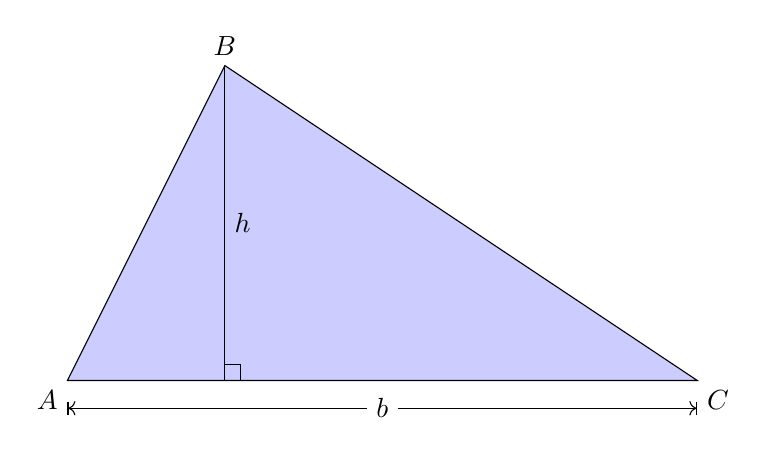
\begin{tikzpicture}

\coordinate (A) at (0,0);
\coordinate (B) at (2,4);
\coordinate (C) at (8,0);

\draw [fill=FilledSurfaceGroupOne] (A) node [below left]{$A$}
      -- (B) node [above]{$B$}
      -- (C) node [below right]{$C$}
      -- cycle;

      \draw[color = black,|<->|] ($(A)!10pt!-90:(C)$) to node [fill=white, midway] {$b$} ($(C)!10pt!90:(A)$);

      \coordinate (Bproj) at (B |- A);
      \draw (B) -- node [right] {$h$} (Bproj);
      \path pic [draw,angle radius=2mm] {right angle = B--Bproj--C};

\end{tikzpicture}
\end{document}

% 
